\documentclass[titlepage = firstcover]{scrartcl}
\usepackage[aux]{rerunfilecheck}
\usepackage{fontspec}
\usepackage[main=ngerman, english, french]{babel}

% mehr Pakete hier
\usepackage{expl3}
\usepackage{xparse}

%Mathematik------------------------------------------------------
\usepackage{amsmath}   % unverzichtbare Mathe-Befehle
\usepackage{amssymb}   % viele Mathe-Symbole
\usepackage{mathtools} % Erweiterungen für amsmath
\usepackage[
  math-style=ISO,    % \
  bold-style=ISO,    % |
  sans-style=italic, % | ISO-Standard folgen
  nabla=upright,     % |
  partial=upright,   % /
]{unicode-math}% "Does exactly what it says on the tin."
\usepackage[section, below]{placeins}

% Laden von OTF-Mathefonts
% Ermöglich Unicode Eingabe von Zeichen: α statt \alpha

\setmathfont{Latin Modern Math}
%\setmathfont{Tex Gyre Pagella Math} % alternativ zu Latin Modern Math
\setmathfont{XITS Math}[range={scr, bfscr}]
\setmathfont{XITS Math}[range={cal, bfcal}, StylisticSet=1]

\AtBeginDocument{ % wird bei \begin{document}
  % werden sonst wieder von unicode-math überschrieben
  \RenewDocumentCommand \Re {} {\operatorname{Re}}
  \RenewDocumentCommand \Im {} {\operatorname{Im}}
}
\usepackage{mleftright}
\setlength{\delimitershortfall}{-1sp}


%Sprache----------------------------------------------------------
\usepackage{microtype}
\usepackage{xfrac}
\usepackage[autostyle]{csquotes}    % babel
\usepackage[unicode, pdfusetitle]{hyperref}
\usepackage{bookmark}
\usepackage[shortcuts]{extdash}
%Einstellungen hier, z.B. Fonts
\usepackage{booktabs} % Tabellen



\title{Wiederholungsaufgaben}
\author{
  Lasse Sternemann\\
  \href{mailto:lasse.sternemann@udo.edu}{lasse.sternemann@udo.edu}
}
\date{Bearbeitet am 20.04.2020}

\begin{document}
    
    \maketitle
    \newpage
    \tableofcontents
    \newpage


    \section{Begriffswiederholung}
        \subsection{Mittelwert}
            Der Mittelwert ist der Durschnitt der Werte einer Wertereihe, die zum Beispiel Messwerte beinhalten kann. Der Mittelwert $\langle x \rangle$ einer 
            Messgröße wird dann berechnet, indem alle Messwerte $x_i$ aufsummiert werden und diese Summe durch die Anzahl $N$ der Messwerte geteilt wird.

            \begin{equation}
                \text{Mittelwert:} \qquad \langle x \rangle = \frac{1}{N} \cdot \sum_{i=1}^N x_i
                \label{eqn:Mittelwert} 
            \end{equation}
            

        \subsection{Standardabweichung}
            Die Standardabweichung $\sigma$ einer Messreihe wird berechnet, um die Streuung der einzelnen Messwerte anzugeben.
            
            \begin{equation}
                \text{Standardabweichung:} \qquad \sigma = \sqrt{\frac{1}{\left(N-1\right)}\cdot \sum_{i=1}^N \left(x_i - \langle x \rangle \right)^2}
            \end{equation}
            
            \noindent Wenn die Standardabweichung groß ist, sind die Messwerte weit um den Mittelwert gestreut. Ist die Standardabweichung jedoch gering, 
            sind die Messwerte eng um den Mittelwert verteilt.

        \subsection{Streuung der Messwerte und Fehler des Mittelwerts}
            Die Streuung der Messwerte kann durch die Standardabweichung betrachtet werden, da diese angibt, wie weit die einzelnen Werte durchschnittlich vom
            Mittelwert entfernt sind. Der Fehler des Mittelwerts $s$ unterscheidet sich durch den Faktor $N^{-(\frac{1}{2})}$ von der Standardabweichung. Dabei ist 
            $N$ wieder der Umfang der Probe. 
            \begin{equation}
                s = \sqrt{\frac{\sum_{i=1}^N \left(x_i - \langle x \rangle \right)^2}{N(N-1)}}
            \end{equation}

    \newpage
    \section{Volumen eines Hohlzylinders}
            Um das Volumen eines Hohlzylinders mit einem Innenradius $R_{\text{I}}$ und Außenradius $R_{\text{A}}$ zu berechnen, muss das Volumen des kleineren Zylinders von dem des Größeren
            abgezogen werden. Dies wird in Formel \ref{eqn:Volumen} getan.
            
            \begin{equation}
                V = \pi h \cdot (R_{\text{A}}²-R_{\text{I}}²)
                \label{eqn:Volumen}
            \end{equation}

            \noindent Da die gegebenen Werte \ref{eqn:Werte} fehlerbehaftet sind, muss über die Gauß'sche Fehlerfortpflanzung \ref{eqn:Gauß} auch der Fehler des 
            Volumens berechnet werden.

            \begin{equation}
                \Delta f = \sqrt{\sum_{i=1}^N \left(\frac{df}{dy_i} \cdot \Delta y_i\right)^2}
                \label{eqn:Gauß}
            \end{equation}

            \noindent Wird die Gauß'sche Fehlerfortpflanzung \ref{eqn:Gauß} auf die Formel des Volumens \ref{eqn:Volumen} unter Berücksichtigung der fehlerbehafteten 
            Größen $R_{\text{I}}$, $R_{\text{A}}$ und $h$ angewendet ergibt sich folgende Formel für den fortgepflanzten Fehler:

            \begin{equation}
                \Delta V = \sqrt{(\pi \cdot (R_{\text{A}}^2-R_{\text{I}}²)\cdot \Delta h)² + (2 \pi h \cdot \Delta R_{\text{A}}^2)² + (-2\pi h \cdot \Delta R_{\text{I}}²)²}
                \label{eqn:FehlerVolumen}
            \end{equation}

            \noindent Wenn die gegebenen Werte

            \begin{equation}
                R_{\text{I}}=(10\pm1)cm \qquad  R_{\text{A}}=(15\pm1)cm \qquad h = (20\pm1)cm
                \label{eqn:Werte}
            \end{equation}

            \noindent nun in die Formeln \ref{eqn:Volumen} und \ref{eqn:FehlerVolumen} eingesetzt werden, ergibt sich das Volumen des Hohlzylinders als

            \begin{equation*}
                V = (7900 \pm 2300) cm³ .
            \end{equation*}

            \noindent Dies entspricht einem prozentualen Fehler von ca. $\pm 29 \% $.

    
    \newpage
    \section{Lineare Regression}
        Bei einem Experiment wurde an verschiedenen Linien eine Spannung gemessen. Aus dieser Messreihe soll ein Diagramm angefertigt werden. Zunächst werden 
        dazu die Linien durch Formel \ref{eqn:D} in Abstände in mm umgerechnet.

        \begin{equation}
            D = (N_{\text{Linie}}-1) \cdot 6 \text{mm}
            \label{eqn:D}
        \end{equation}
        
        \begin{table}[h]
            \centering
            \label{tab:Messwerte}
            \begin{tabular}{c c c}
                \toprule
                {Linie} & {D \ [mm]} & {U \ [V]} \\
                \midrule
                0       & 0          & -19,4     \\
                1       & 6          & -16,1     \\
                2       & 12         & -12.4     \\
                3       & 18         & -9.6      \\
                4       & 24         & -6.2      \\
                5       & 30         & -2.4      \\
                6       & 36         & 1.2       \\
                7       & 42         & 5.1       \\
                8       & 48         & 8.3       \\
                \bottomrule                
            \end{tabular}
            \caption{Der direkten Messung entsprechen die Wertepaare aus Linie und Spannung U. Die mittlere Zeile D wurde über Formel \ref{eqn:D} aus den Werten der Liniensäule berechnet und gibt einen Abstand an.}
        \end{table}
        
        \noindent Nun werden die Werte von D gegen die von U aufgetragen und eine lineare Regression angefertigt. Diese beruht auf der Geradengleichung

        \begin{equation*}
            D = m\cdot U + b
        \end{equation*}

        \noindent mit den Parametern

        \begin{align}
            m &= (1,72 \pm 0,02) \frac{mm}{V} \\
            b &= (33,86 \pm 0,22) mm.
            \label{eqn:Parameter}
        \end{align}

        \begin{figure}
            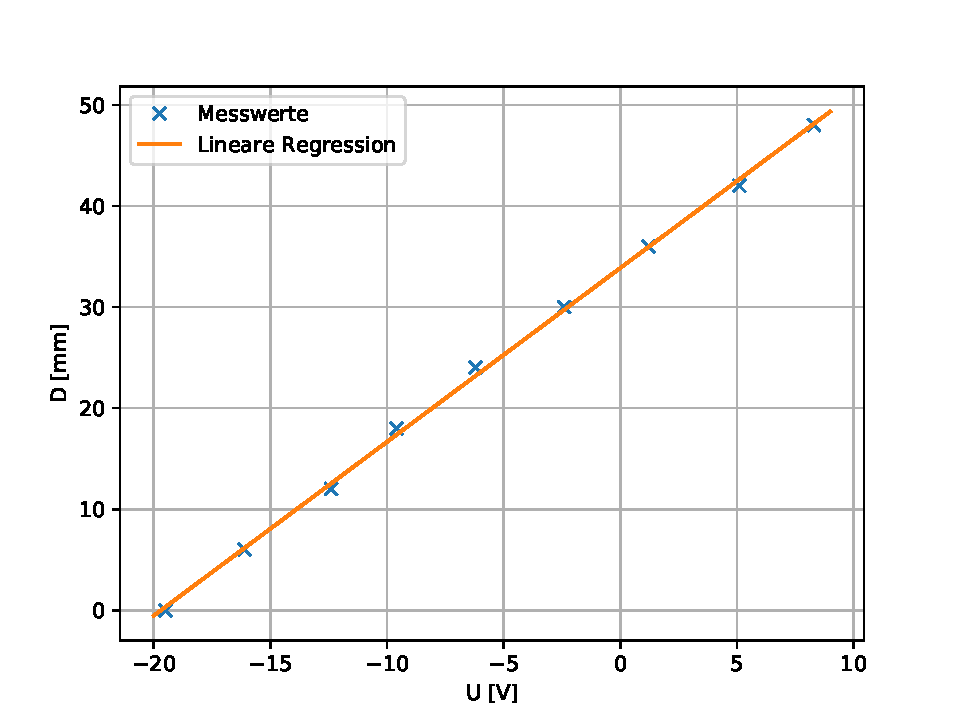
\includegraphics{UD_plot.pdf}
            \caption{In der Grafik sind die Abstände D gegen die Spannungen U aufgetragen. Zudem wird eine linerae Regression aus den Wertepaaren gebildet und über die Messwerte gelegt. Die Parameter der linearen Regression \ref{eqn:Parameter} sind oben aufgeführt.}
            \label{fig:Graf}
        \end{figure}

\end{document}